\chapter{Analysis with the Full Run 2 Dataset}
\label{chapter:fullRun2}

% --------------------------------------------------------------------------------------
\section{Event Selection Optimization}

For the full Run 2 analysis the event selection for the signal region will need to be reoptimized. In practice this is done by defining multiple potential signal regions with each cut varied in intervals (e.g. \etmiss > 80, 85, 90, 95, 100, ... GeV). Then in each region the signal significance $Z$ is calculated. The formula used in the past iterations of the analysis is given by \cite{Cowan1}:

\begin{equation}
Z = \sqrt{2 \left( (s+b) \ln \left( 1+\frac{s}{b} \right) -s \right)} 
\label{eqn:Z1}
\end{equation}

\noindent $s$ and $b$ are the expected number of signal and background events in MC, and $s+b$ follows a Poisson distribution. If $s \ll b$ then the formula reduces to $Z = s/\sqrt{b}$. The main caveat with this formula however is that the uncertainty on $b$ is considered to be negligible. If one takes the uncertainty on $b$ to be $\sigma_b$, then the formula becomes \cite{Cowan1}:

\begin{equation}
Z = \sqrt{2 \left( (s+b) \ln \left( \frac{(s+b)(b+\sigma_b^2)}{b^2+(s+b)\sigma_b^2} \right) - \frac{b^2}{\sigma_b^2} \ln \left( 1 + \frac{\sigma_b^2 s}{b(b+\sigma_b^2)} \right) \right)} 
\label{eqn:Z2}
\end{equation}

\noindent This formula reduces to $Z = s/\sqrt{b+\sigma_b^2}$ for $s \ll b$ and $\sigma_b^2 \ll b$. Using this formula would be an improvement compared to using Equation \ref{eqn:Z1}. The significance is estimated from MC, so the uncertainties $\sigma_b$ could be either (a) the experimental systematics as applied to the MC, or possibly (b) approximated from the much larger data-driven uncertainties on the background estimates from the 2015+2016 dataset. These uncertainties were calculated in a specific signal region, but their approximate magnitudes could be useful for estimating a more correct significance. 

A reoptimization of the signal region is also motivated by newly available \etmiss-related quantities that could improve the \monoZ analysis. For example, two \etmiss working points are now available. In the new ``tight'' \etmiss definition, jets in the forward region of the detector must have \pt > 30 GeV to reduce contributions from pileup. The ``loose'' definition (used previously in this analysis) includes all jets with \pt > 20 GeV except for forward jets with \pt < 60 GeV that fail an additional minimum jet vertex tagger requirement, a multivariate criteria that identifies pileup jets from tracks. The tight definition is now recommended because the \etmiss resolution is improved. Both definitions will be studied to validate the improvement in switching to the tight definition.

There is also now the option to use particle-flow \etmiss, which is calculated using particle-flow jets. The particle-flow algorithm \cite{Sirunyan:2017ulk} uses information from both the tracker and the calorimeter to determine the energy of a jet. Traditional jets are constructed only using energy deposits in the calorimeter. The tracker has better energy resolution than the calorimeter (for particles with low momentum), better angular resolution, and can better detect soft charged particles that may not meet the noise threshold of the calorimeter. Particle-flow jets may be a better option for calculating a more reliable \etmiss, especially in higher pileup conditions. Particle-flow \etmiss will need to be studied and compared with the traditional \etmiss to determine which is better suited for the analysis.

Another new variable is the \etmiss significance $\mathcal{S}$ \cite{Schaefer:2294922}. It is defined using a log-likelihood ratio and quantifies how likely it is that the reconstructed \etmissvec is consistent with genuine \etmissvec $\neq 0$ (i.e.\ that there are real invisible particles in the event, as opposed to a non-zero \etmissvec from particle measurement resolution and efficiency effects). It is defined as

\begin{equation}
\mathcal{S}^2 = 2 \ln \left( \frac{\mathcal{L}(\vec{E}_\text{T}^\text{miss} | \vec{p}_\text{T}^\text{ inv} \neq 0)}{\mathcal{L}(\vec{E}_\text{T}^\text{miss} | \vec{p}_\text{T}^\text{ inv} = 0)} \right),
\end{equation}

\noindent where $\vec{p}_\text{T}^\text{ inv} = -\vec{E}_\text{T}^\text{miss}$. A large $\mathcal{S}$ indicates that the \etmissvec is not well explained by resolution smearing effects, and real invisible particles are likely to be in the event. This discriminant is more powerful in rejecting events with fake \etmiss from mis-measured objects (compared to more traditional variables such as \etmissht) because it includes the uncertainties of the reconstructed objects and track-based soft term that enter the \etmiss calculation. Hence this is a promising variable to help reduce the \Zjets background, arguably the most difficult background to estimate in this analysis.

Finally, an added complication in the future event selection optimization of the analysis is the potential for multiple signal regions. As we study more varieties of dark matter models, the cuts that optimize the significance for different signals may differ. If the significance for different signals varies greatly with different cuts, it may be optimal to have more than one signal region. However, this adds additional challenges to the analysis, such as having to estimate backgrounds in multiple regions; if a background is difficult to estimate (e.g. large correlations when estimating \Zjets with the ABCD method), this can increase the amount of time needed to validate the technique and obtain a reasonable data-driven estimate. Since the analysis has limited manpower, it may be decided to have a slightly sub-optimal signal region and sacrifice some significance. These types of decisions will have to be discussed in the group moving forward.


% --------------------------------------------------------------------------------------
\section{Development of the \gjets Technique}

The \gjets method for estimating the \Zjets background is under development. For the 2015+2016 dataset, a heavily modified ABCD method was used for the \Zjets data-driven estimate. The systematic errors on the estimate were large, on the order of 50-100\%. It would be desirable to have a more reliable estimate for this background from the \gjets method for the full Run 2 result.

As discussed in Section \ref{sec:gjets}, for the 2015+2016 dataset acceptable agreement was obtained between MC \gjets and \Zjets events in the signal region, with the estimates nearly agreeing within statistical errors. The method used a 2x1D reweighting scheme with the boson \pt and the \etmissht. After the reoptimization of the event selection, this scheme may change. For example, with the introduction of the \etmiss significance described in the previous section, it may be better to redo the \gjets estimate with \pt and $\mathcal{S}$, that is if $\mathcal{S}$ is chosen to be included in the event selection. Depending on the selections chosen, it could be worth reinvestigating a few of the more promising pairs of variables with which to perform the reweighting. In addition, the improved statistics of the Run 2 dataset may provide opportunity for more reliable 2D weights, but this will need to be assessed. It may also be worthwhile to investigate the effects of the reweighting before/after certain cuts. For example, the largest disagreement between \gjets and \Zjets events in the cutflow was seen at the \etmiss (and \etmissht) cut. It could be that reweighting the events after the \etmiss requirement may help to improve the agreement.

Once acceptable agreement is seen in \gjets and \Zjets events, the next step would be to apply the method to data. A few methods for doing this have been discussed. For example, should the weights be obtained from data or MC? This may depend on which has more reliable statistics. The validation of the weights must also be tested, for example by applying weights obtained in MC to data and then looking at the agreement with the reweighted MC. Differences seen in the agreement must then be quantified as systematic errors in the technique. 

There is also the technical side of implementing the \gjets technique in the MonoZUVic software. This was done previously for the 2015+2016 dataset, but since then the code has undergone a significant redesign, and the \gjets estimate will need to be reimplemented.

% --------------------------------------------------------------------------------------
\section{Signal Models}

More dark matter models with be studied in the \monoZ analysis with the full Run 2 dataset. As recommended by the LHC DM Working Group, $s$-channel simplified models with spin-0 mediators will continue to be the benchmark model used in the analysis; however signals will be simulated at next-to-leading order (NLO) in QCD rather than LO, as higher-order QCD corrections have been shown to have a significant impact on the production rate and kinematic distributions of these models \cite{Backovic:2015soa}. In addition, these models allow for mediator couplings to leptons. In total there are four NLO benchmark scenarios recommended \cite{Albert:2017onk} with the following couplings:

\begin{table}[h]
\centering
\begin{tabular}{ccccc}
\hline \hline
Model & Mediator     & $g_q$ & $g_\ell$ & $g_\chi$ \\ \hline \hline
A1    & axial-vector & 0.25  & 0.0      & 1.0      \\ \hline
A2    & axial-vector & 0.1   & 0.1      & 1.0      \\ \hline
V1    & vector       & 0.25  & 0.0      & 1.0      \\ \hline
V2    & vector       & 0.1   & 0.01     & 1.0    \\ \hline \hline
\end{tabular}
\caption{Benchmarks for NLO $s$-channel simplified models in Run 2.}
\label{tbl:nloSimp}
\end{table}

\noindent Recent work \cite{ChrisA} has shown that it is possible to rescale from A1 to A2 and V1 to V2 using the ratio of cross sections. We are currently working on sample requests for the A1 and V1 models, and scaling will be done for the A2 and V2 scenarios. Mass point emulation will also be carried out again to reduce the number of reconstructed samples needed. The full Run 2 dataset is expected to be $\sim$140 \ifb. To estimate how the limits will improve for such a dataset, the NLO limits obtained with 36.1 \ifb have been scaled to an integrated luminosity of 140 \ifb. Figure \ref{fig:140limits} shows a projection for the NLO axial-vector limits \cite{ChrisA}. This projection assumes the same signal region and background estimates as used for the 2015+2016 dataset. These will of course change with the full dataset, but it gives an estimate for the masses at which we should request samples. Compared to 36.1 \ifb (as in Figure \ref{fig:limits}), the expected reach in \mmed improves from 550 GeV to nearly 900 GeV for light \mchi, and the maximum reach in \mchi improves from 250 GeV up to 350 GeV.

\begin{figure}[!htb]
\centering
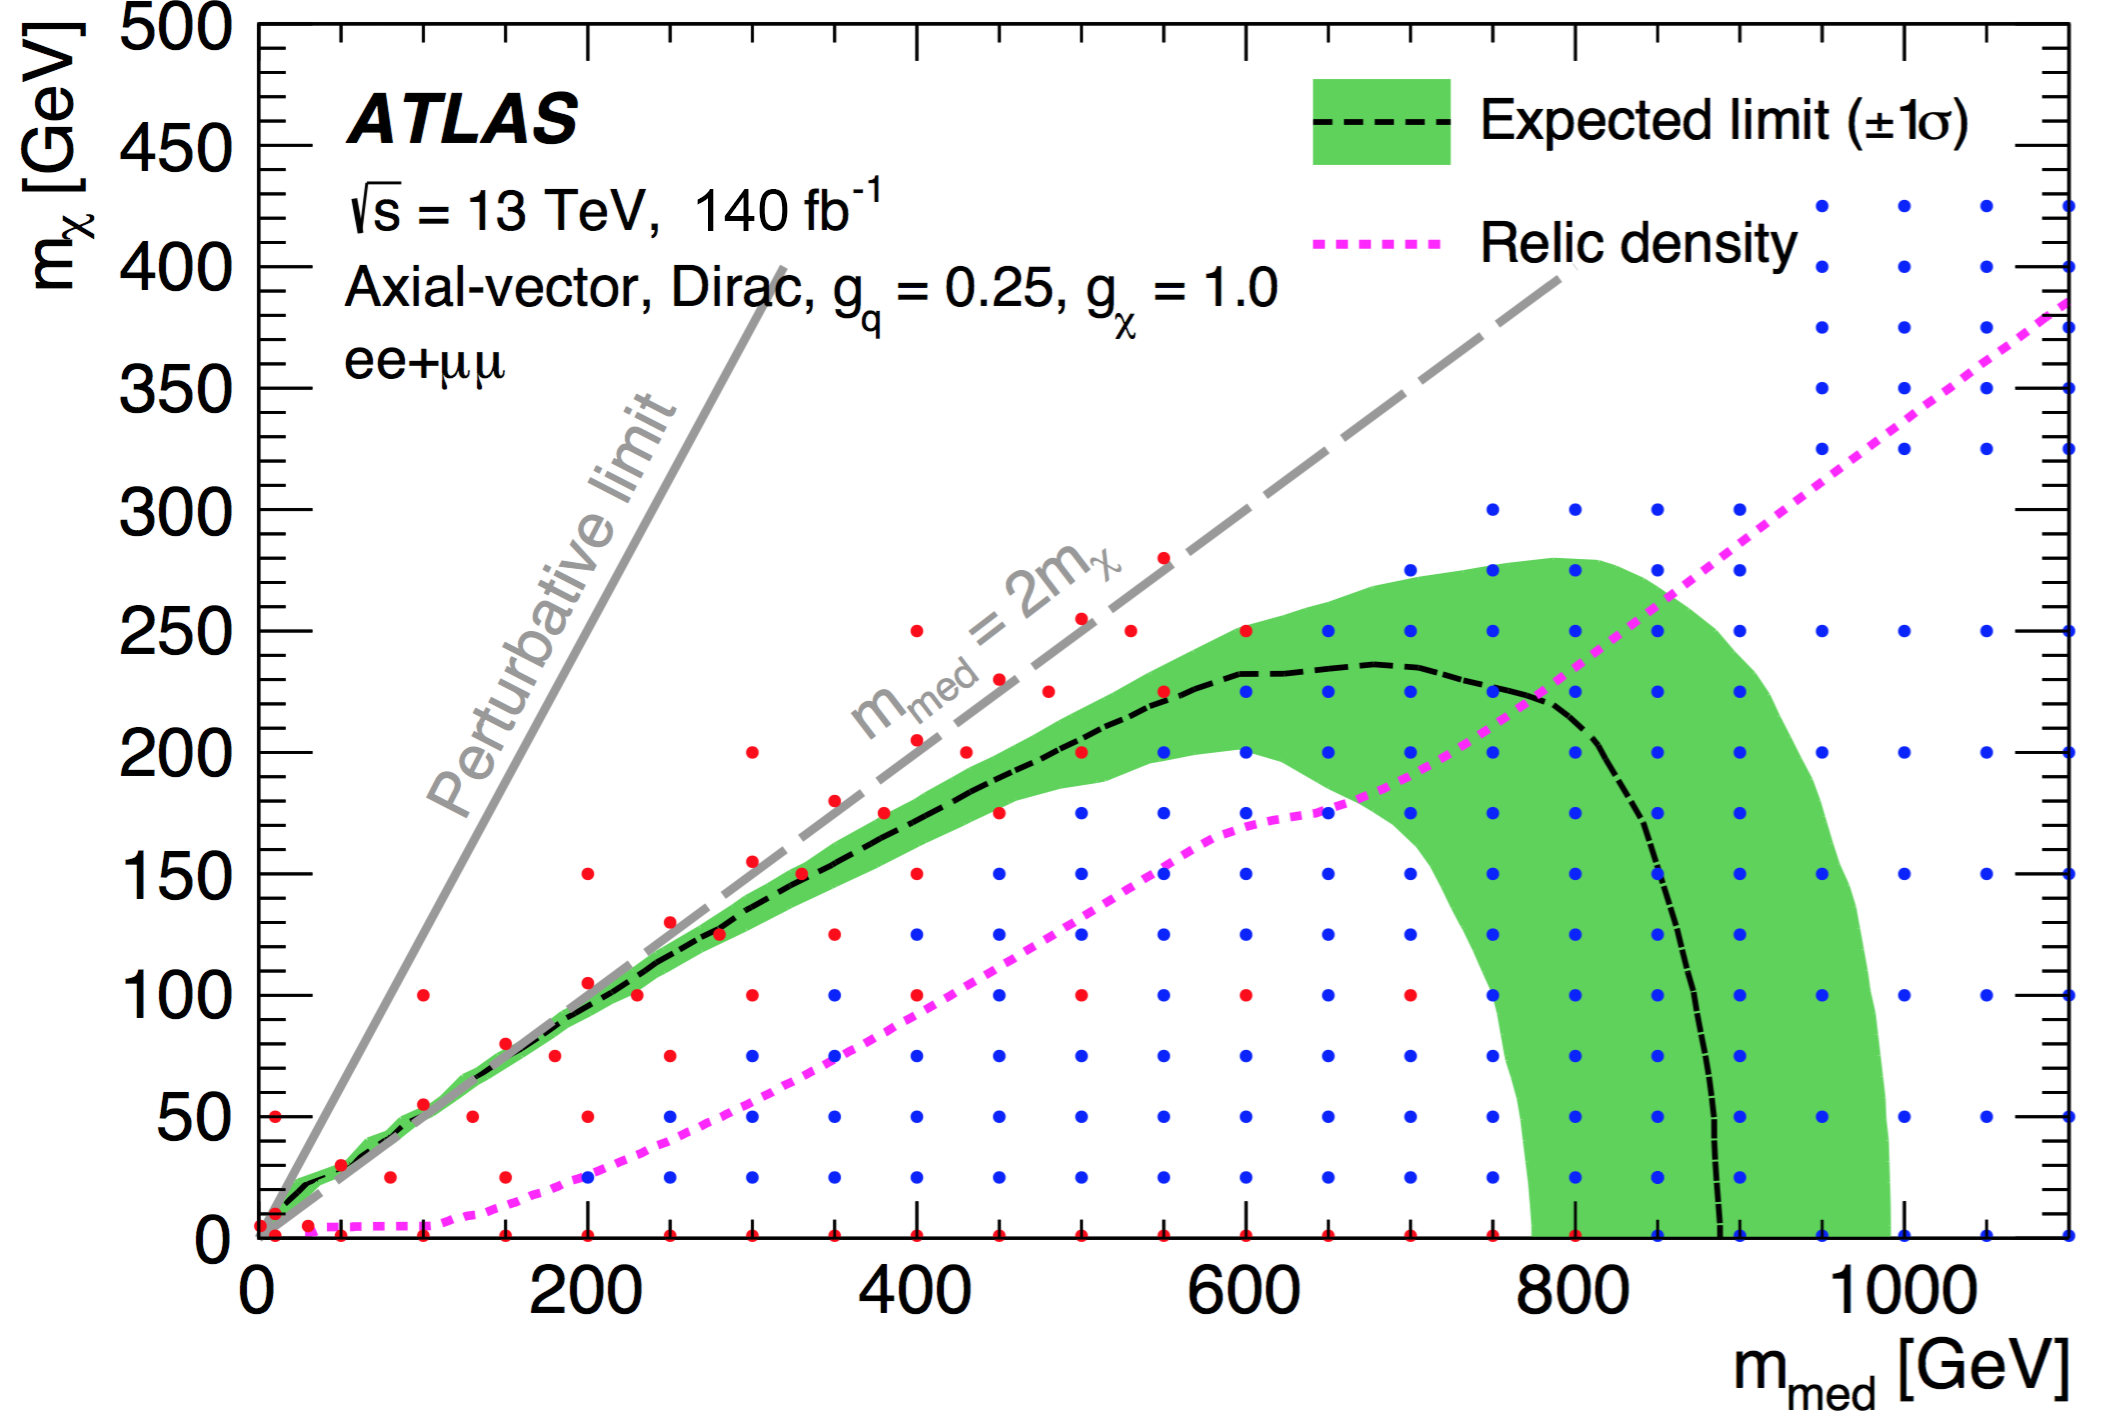
\includegraphics[width=0.7\textwidth]{Figures/140ifb.png}
\caption{Prospective NLO $s$-channel axial-vectorvector exclusion limit with 140 \ifb \cite{ChrisA}.}
\label{fig:140limits}
\end{figure}

In addition to the simplified models, the 2HDM+PS model has become a new standard in the analysis. A similar projection to 140 \ifb will be done using the limits on $m_H$ vs $m_a$ and $\tan \beta$ vs $m_a$ with 36.1 \ifb shown in Section \ref{sec:limits}, and a request for more reconstructed samples will follow suit. Mass point emulation for the 2HDM+PS model is more complicated than for the simplified models; both the signal acceptance and the \etmiss shape depend non-trivially on $m_a$ and $m_H$, and the best method for emulating samples is still being investigated.

The other type of signature to be investigated with the full Run 2 dataset is the $t$-channel signature with a coloured scalar mediator. There are various models that encompass this type of signature (Figure \ref{fig:tchan_bell} shows the relevant $t$-channel diagrams for \monoZ). A few potential models to be considered are discussed here. These models are of interest for the \monoZ search because the $Z$ is allowed to couple directly to the mediator, a channel unique to \monoZ.

\begin{figure}[!htb]
\centering
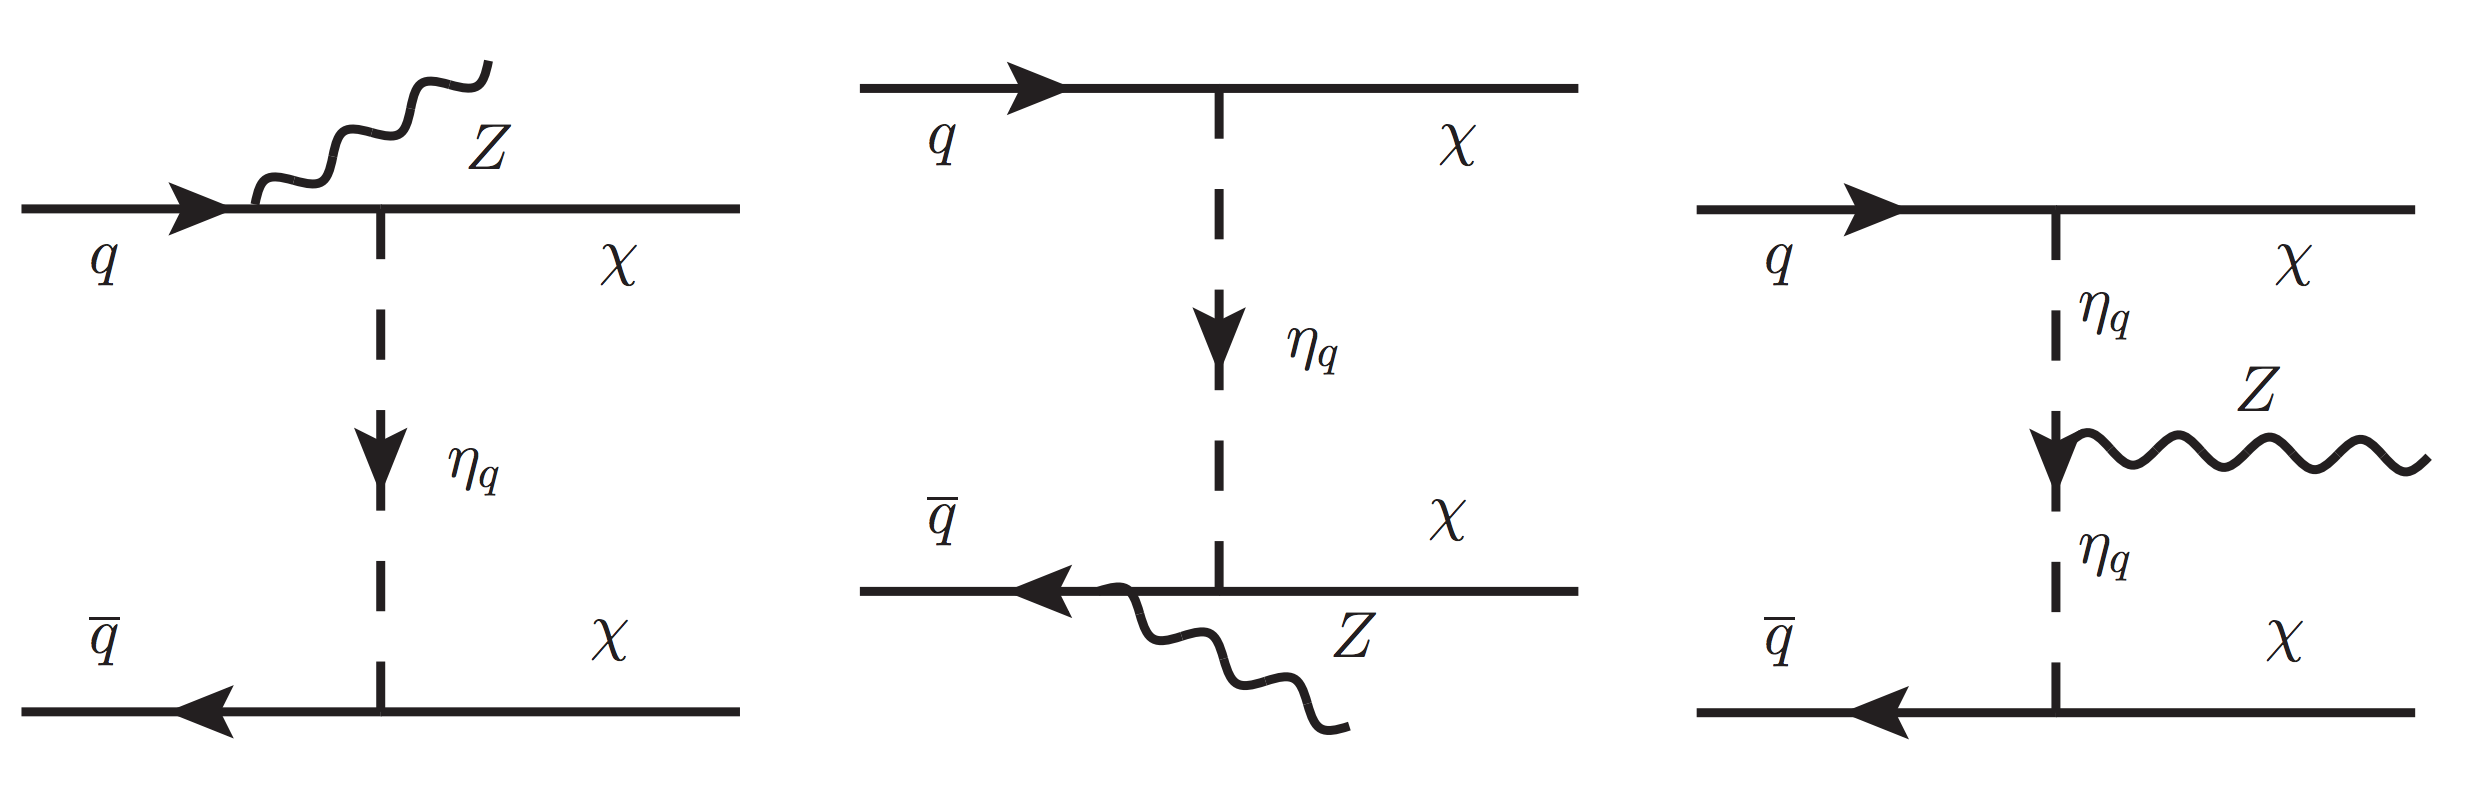
\includegraphics[width=0.75\textwidth]{Figures/tchan_bell.png}
\caption{$t$-channel diagrams with the \monoZ signature \cite{Bell:2012rg}.}
\label{fig:tchan_bell}
\end{figure}

The Papucci model \cite{Papucci:2014iwa} was the first $t$-channel model recommended by the LHC DM WG in Ref.\ \cite{Abercrombie:2015wmb}. The interaction Lagrangian is given by:

\begin{equation}
\mathcal{L}_\text{int} = g \sum_{i=1,2} \left( \eta_{(i),L} \bar{Q}_{(i),L} + \eta_{(i),u,R} \bar{u}_{(i),R} + \eta_{(i),d,R} \bar{d}_{(i),R} \right) \chi + h.c.
\end{equation}

\noindent Here $Q_{(i),L}$, $u_{(i),R}$, and $d_{(i),R}$ are the SM quarks, $\eta_{(i),L}$, $\eta_{(i),u,R}$, and $\eta_{(i),d,R}$ are the mediator particles, and $g$ is the coupling between the SM particles and dark matter. $L$ and $R$ indicate left- and right-handedness, and the index $i$ is the quark generation. In the Papucci model only the first two generations are considered. 

The mono-jet analysis recently set limits on the $t$-channel signature using the Bell model \cite{Bell:2012rg}, a variant of the Papucci model with the interaction Lagrangian:

\begin{equation}
\mathcal{L}_\text{int} = g \sum_{i=1,2,3} \eta_{(i),L} \bar{Q}_{(i),L} \chi + h.c.
\end{equation}

\noindent In this model, couplings to right-handed quarks are turned off, but the third generation of quarks is included. The mono-jet analysis chose to use this model without including the third generation. This decision was based on the availability of Bell et al.\ to answer technical questions about the implementation/generation in \madgraph. The best choice for the \monoZ search will need to be investigated.

The so-called Less Simplified (LS) models \cite{Ko:2016zxg} are another promising category. These models are similar to simplified models but have the full gauge symmetry of the Standard Model. For this model the interaction Lagrangian between quarks and dark matter for $t$-channel processes is:

\begin{equation}
\mathcal{L}_\text{int} = - \left[ \bar{\chi} \sum_{i=1,2,3} \sum_{j=1,2,3} \left( \tilde{Q}_L^{i\dagger}(\lambda_{Q_L})_i^j Q_{Lj} + \tilde{u}_R^{i\dagger} (\lambda_{u_R})_i^j u_{R_j} + \tilde{d}_R^{i\dagger} (\lambda_{d_R})_i^j d_{Rj} \right) + h.c. \right]
\end{equation}

\noindent In this notation, $\tilde{Q}_{Li}$, $\tilde{u}_{Ri}$, and $\tilde{d}_{Ri}$ are new scalar bosons, partners of the SM particles $Q_{Li} = (u_{Li},d_{Li})^T$, $u_{Ri}$, and $d_{Ri}$. Each interaction depends on the chirality, with couplings $\lambda_{Q_L}$, $\lambda_{u_R}$, and $\lambda_{d_R}$. The dark matter mass $m_\chi$ is another parameter, along with twelve mediator masses (four for each of the three generations). For searches in $pp$ collisions, only the first generation will be relevant, so the mediator masses in the second and third generations are approximated to be heavy. With this assumption and a few other simplifications discussed in Ref.\ \cite{Ko:2016zxg}, the number of free parameters for a first benchmark can be reduced to only four: two couplings $\lambda_{Q_L}$ and $\lambda_{u_R}$, and two masses $m_{Q_L}$ ($= m_{Q_{Lu}} = m_{Q_{Ld}}$) and $m_\chi$. Hence 2D mass exclusion limits could be set for fixed couplings as a first step.

And there are even more models \cite{Bauer:2017fsw} being considered as potential new $t$-channel benchmarks. Discussions are needed with the LHC DM WG in order to determine the best model(s) to investigate.

The Papucci model may serve as a good starting point. The \monoZ analysis currently has eight Papucci model signal samples that were requested at the start of Run 2. Hypothesis tests were run on them with 36.1 \ifb of data, but none of the samples were excluded. The mono-jet analysis recently set $t$-channel exclusion limits using the Bell model, and their axial-vector and coloured scalar mediators exclusion regions were quite similar. Hence it was unexpected that none of the \monoZ signals were excluded. This led to some investigations, revealing that the \monoZ samples were generated with an incorrect mediator width. The plan now is to use \madgraph to generate $t$-channel samples with the correct and incorrect mediators to understand the effect on signal. If only the cross section is affected and not the \etmiss, then it may be possible to scale the incorrect reconstructed samples to the correct normalization and then rerun the limit setting. From the mono-jet analysis we expect to get similar reach in mass as for the axial-vector model. Then an estimate can be made on how far the limit will reach and a full set of $t$-channel samples can be requested. Mass point emulation will also need to be investigated at the same time to determine how fine/coarse the grid of reconstructed points should be. This could be done in tandem with investigating another model, such as the LS model, for which we have already generated our own MC.

% --------------------------------------------------------------------------------------
\section{Other Analysis Improvements}

One improvement on the horizon for the analysis is the inclusion of weights in the official ATLAS signal MC generation to calculate QCD, PDF, and PS systematic uncertainties. This will allow the systematic variations to be calculated for each sample using a weight, rather than having to tediously generate our own truth samples for each variation. This will be especially useful for NLO samples, since MC generation will take much longer than for models at LO. In addition, the uncertainty for each sample will be used rather than having to interpolate between masses, etc. The technical implementation of including these weights in our \madgraph and \pythia simulation has been successful; the weights will be included in the upcoming NLO simplified model sample requests, and hopefully all future requests for other models. The proper procedure for using these weights will need to be studied and the analysis code will need to be adapted accordingly.

\begin{figure}[!htb]
\centering
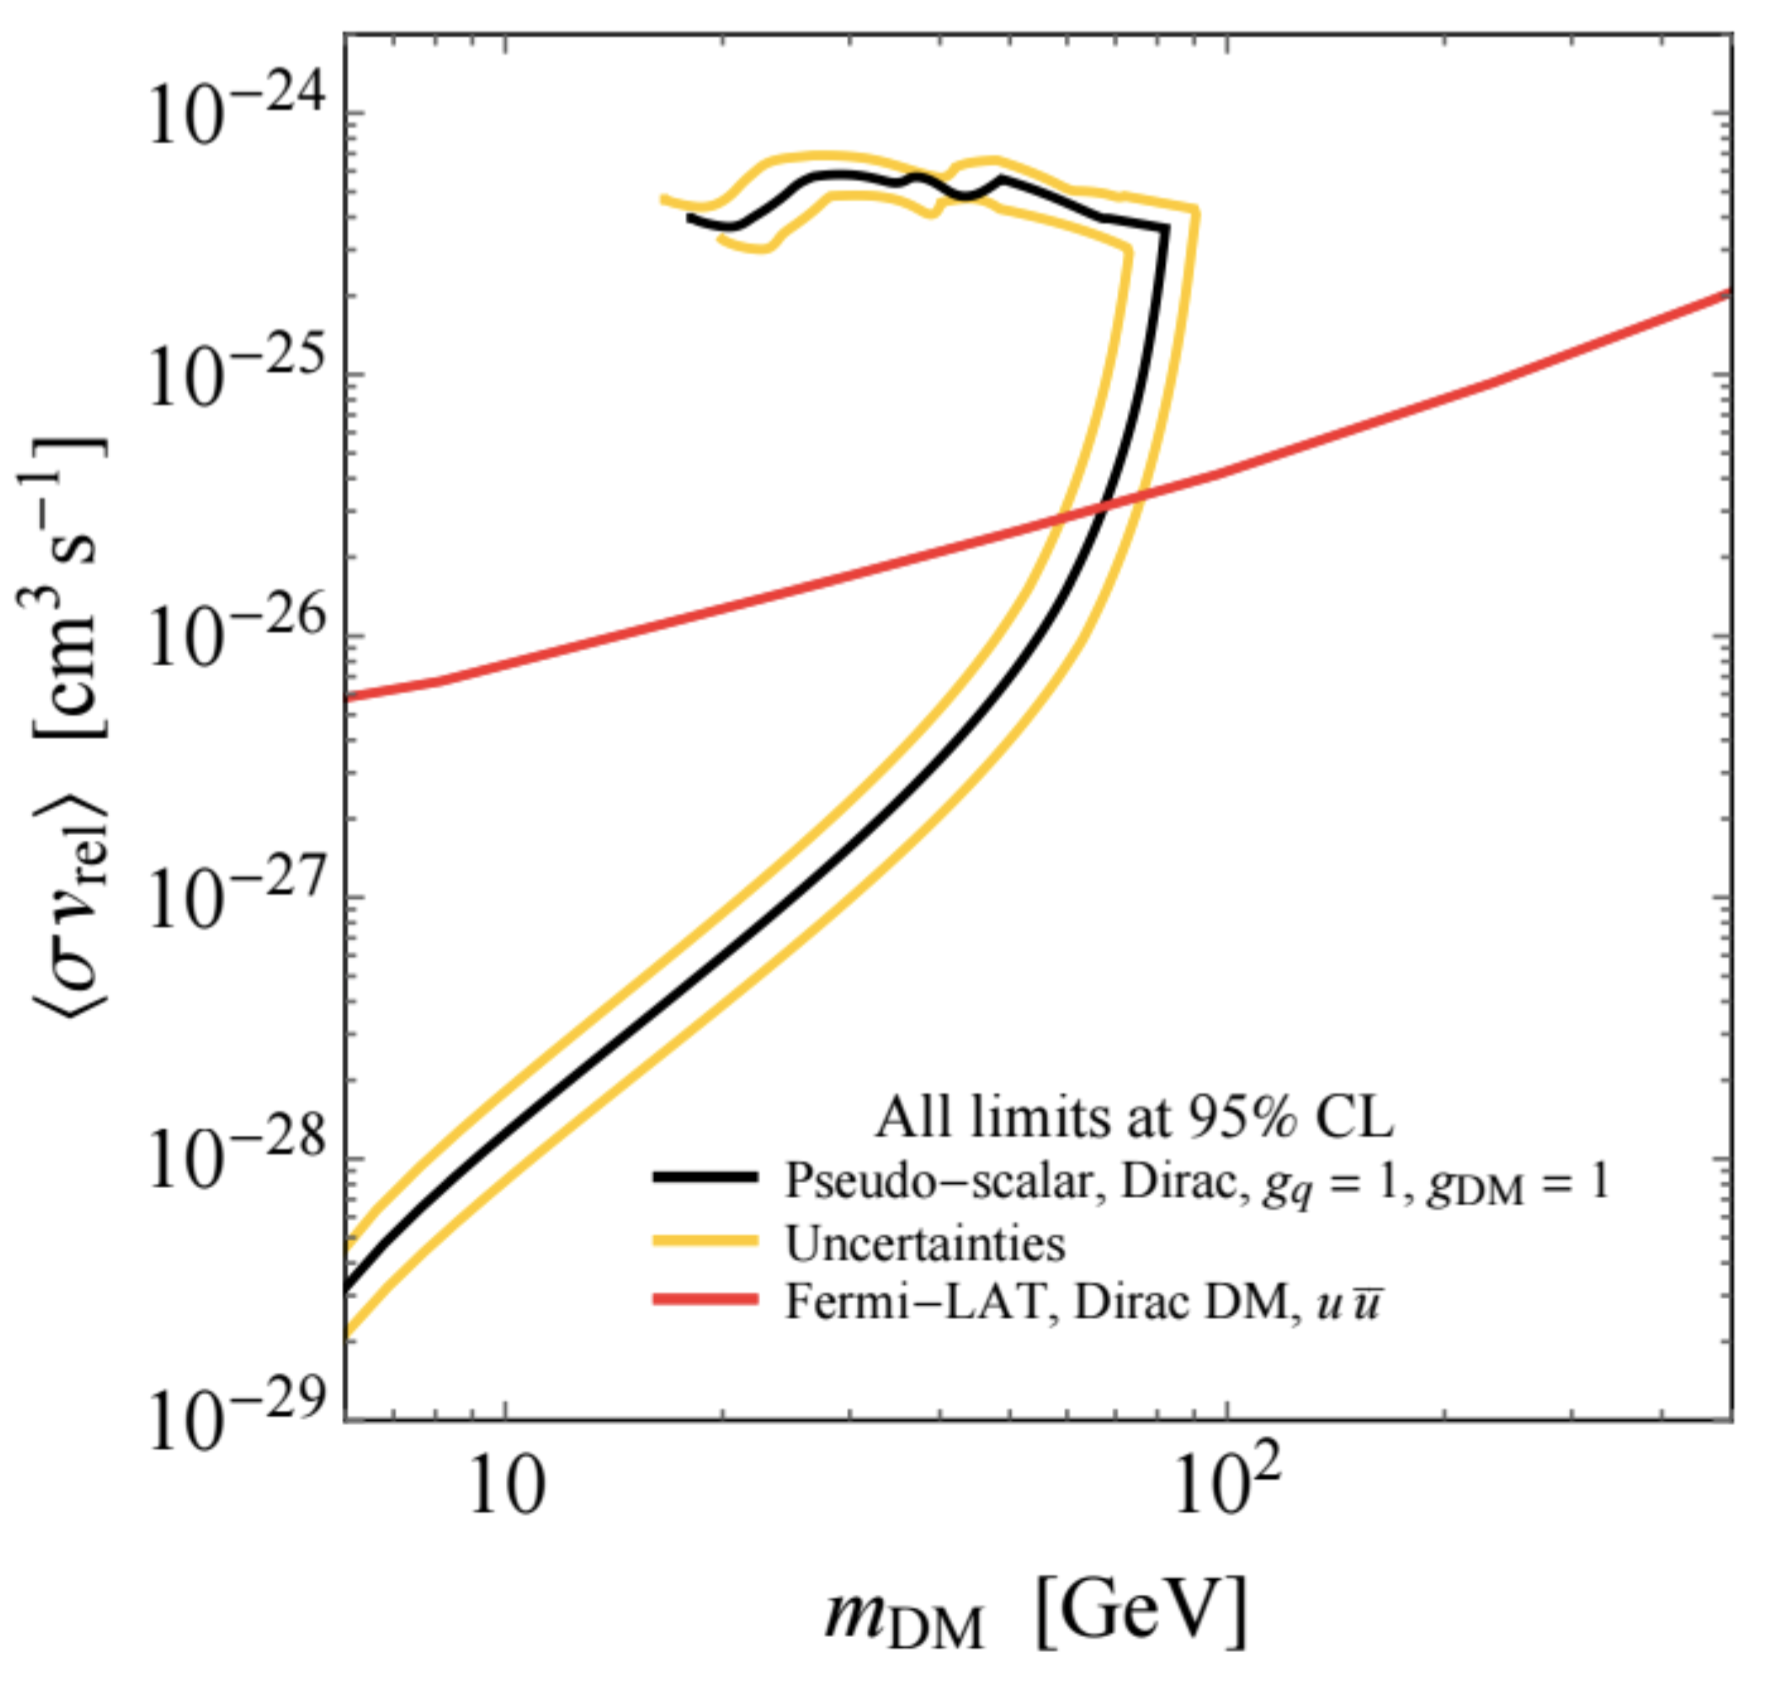
\includegraphics[width=0.5\textwidth]{Figures/id.png}
\caption{Schematic of a collider limit on $\langle \sigma v_\text{rel} \rangle$ overlaid with a ID measurement \cite{Boveia:2016mrp}.}
\label{fig:id}
\end{figure}

\begin{figure}[!htb]
\centering
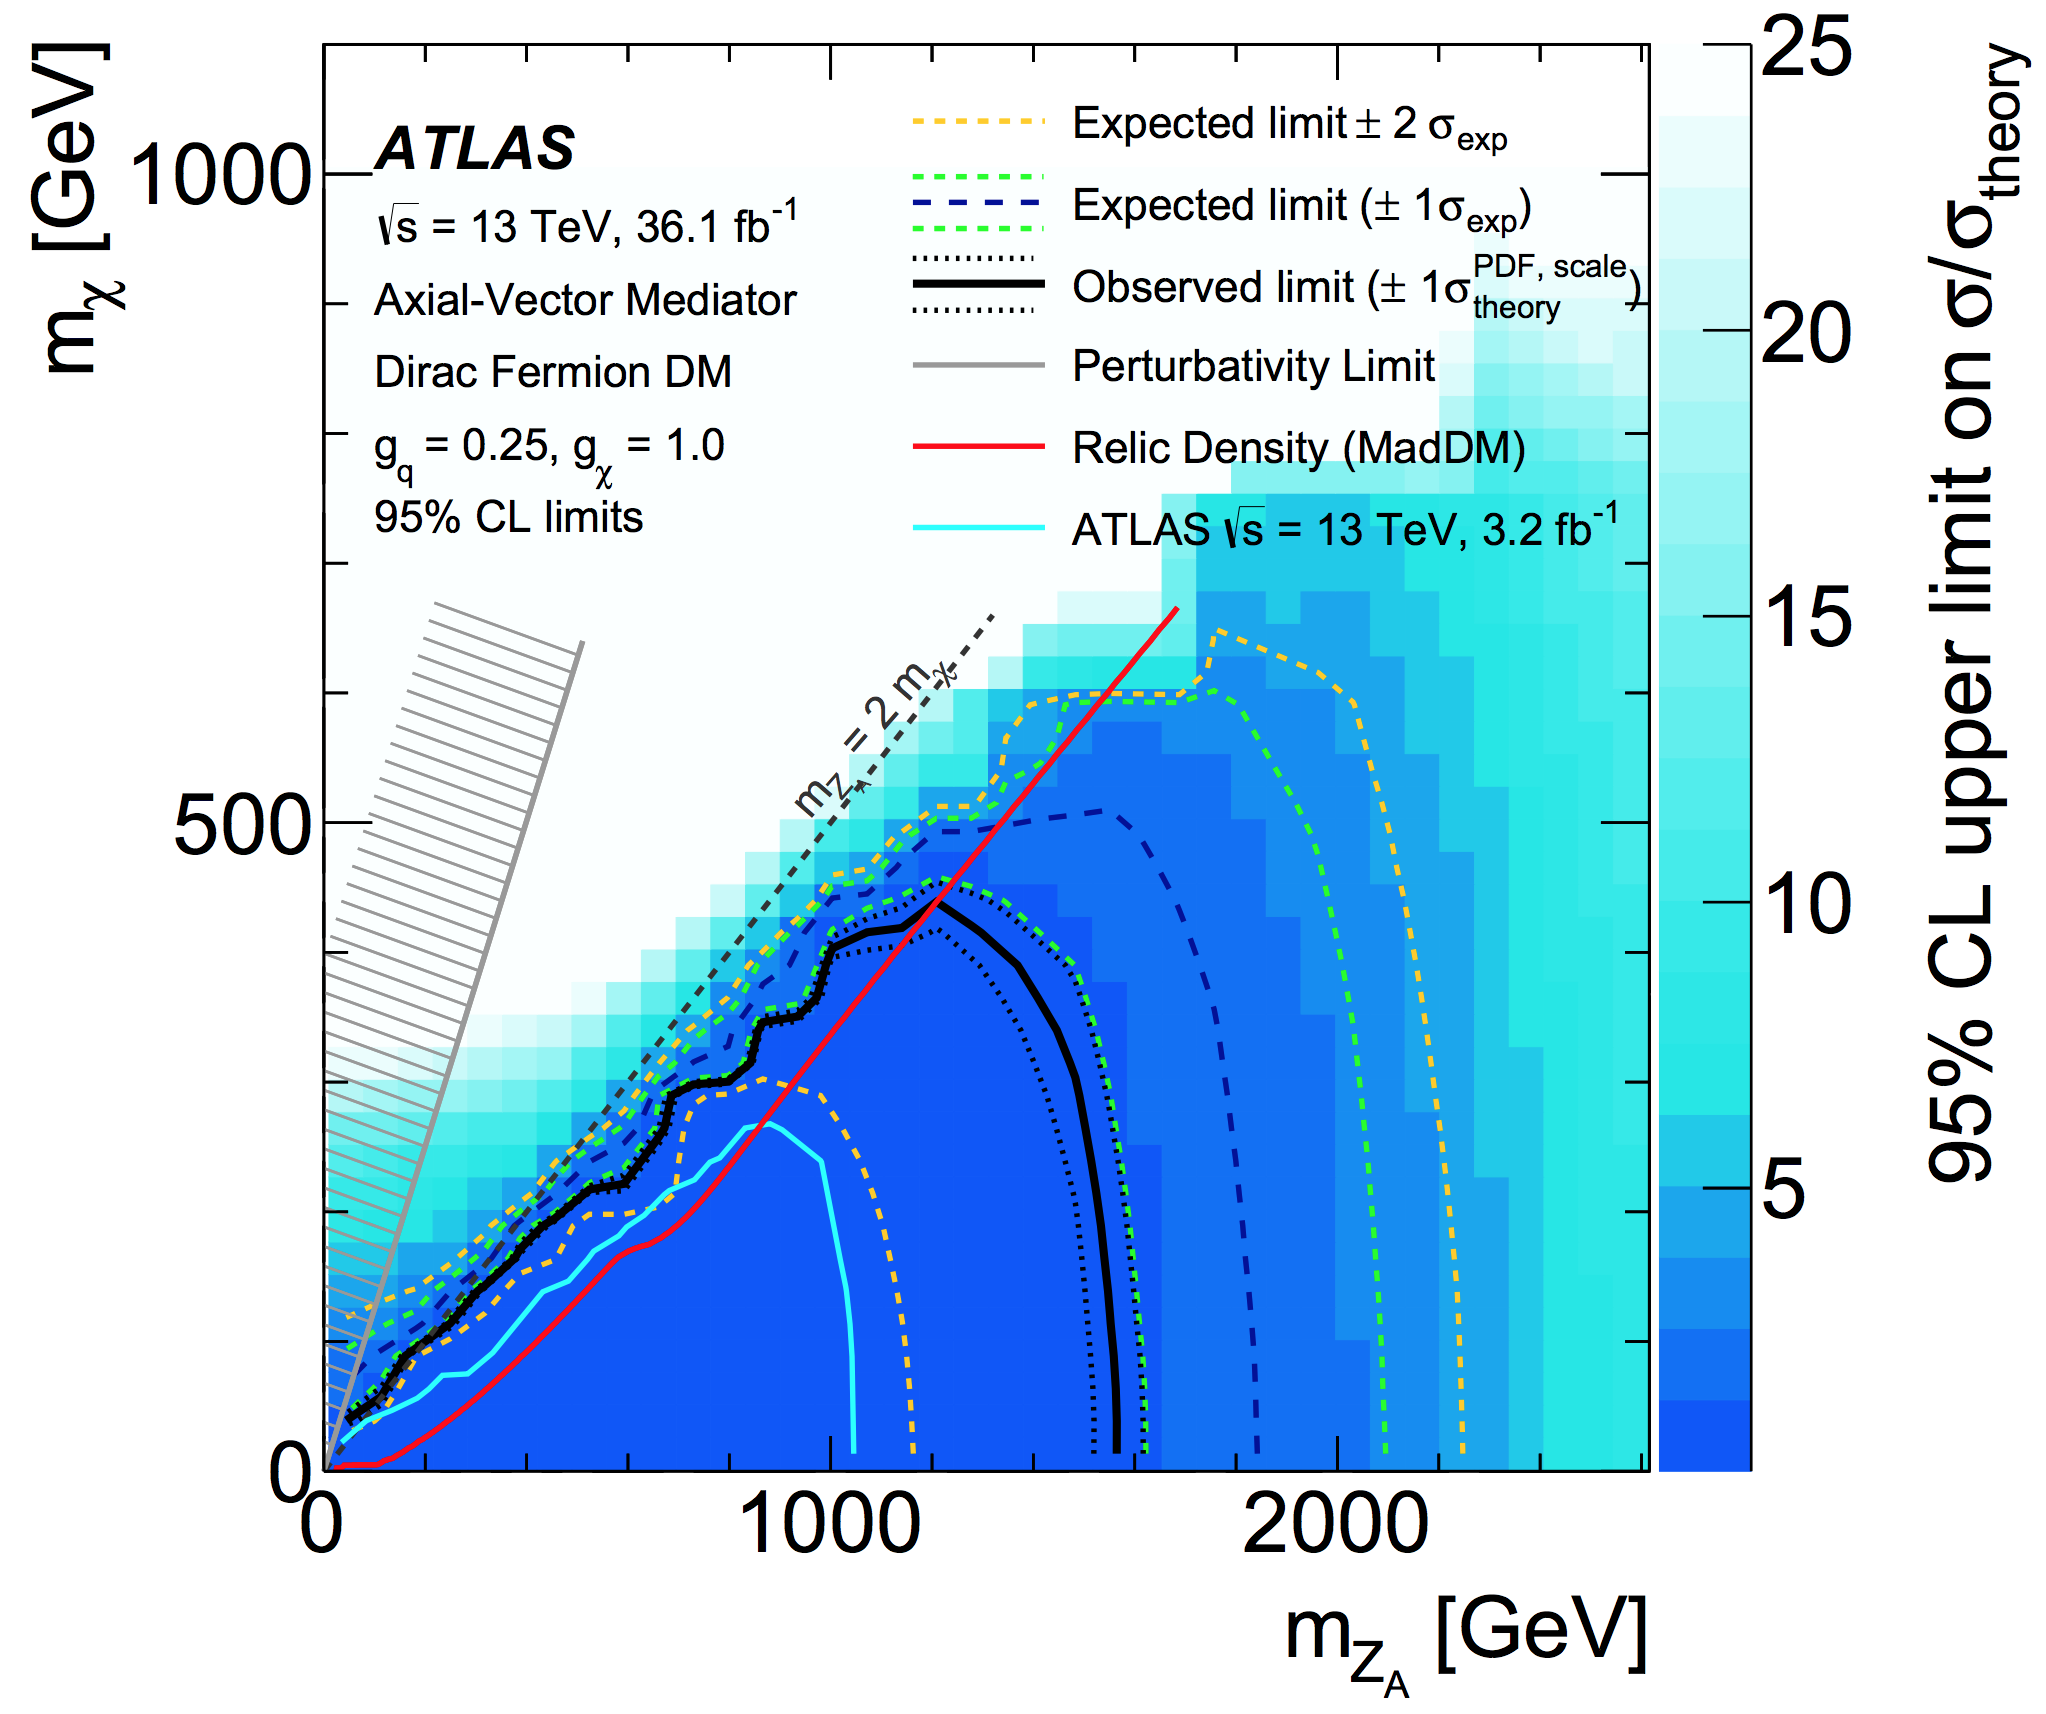
\includegraphics[width=0.6\textwidth]{Figures/limits_dmA_sigma.png}
\caption{Mono-jet axial-vector upper limits on $\mu$ with 36.1 \ifb \cite{Collaboration:2268179}.}
\label{fig:limits_dmA_sigma_monojet}
\end{figure}

There are also a few different interpretations of the \monoZ exclusion limits that remain to be done. For example, the limits have previously been recast into limits on the DM-proton scattering cross section for comparison with direct detection experiments. The same can be done to put limits on the velocity-averaged dark matter annihilation cross section into $q\bar{q}$ and compare with indirect detection experiments. The procedure for converting the 2D mass limits into a limit on $\langle \sigma v_\text{rel} \rangle$ is covered in Ref. \cite{Boveia:2016mrp}. Figure \ref{fig:id} gives a schematic example of such a comparison.

The \monoZ exclusion limits can also be reinterpreted as an upper limit on the dark matter production cross section. The 2D mass exclusions shown in e.g.\ Figure \ref{fig:limits} are determined using the \cls value for a signal strength of $\mu=1$. The observed contour is the line at which \cls = 0.05, and the upper limit on $\mu$ on this line equals 1 by definition. The region within the contour has an upper limit < 1, and the region outside the contour has an upper limit > 1. The upper limit on $\mu$ can hence be used to determine the upper limit on the cross section for the dark matter production process using $\mu \equiv \sigma/\sigma_\text{theory}$, where $\sigma$ and $\sigma_\text{theory}$ are the observed and predicted production cross sections. Figure \ref{fig:limits_dmA_sigma_monojet} shows such a plot from the mono-jet axial-vector search. The colours on the $z$-axis indicate the observed upper limit on $\mu$. The same type of plot can be produced for \monoZ.

Finally, the \monoZ analysis software will continue to be used and improved throughout Run 2. With each new data-taking period, there comes new sets of recommendations on how to use the tools for calibrating objects, apply pileup reweighting, etc.
These recommendations are being finalized for the 2017 data-taking period, and there will be more to come for 2018. The code will continue to be updated and validated throughout the entire Run 2 campaign.

